% simulations
We use simulations to provide additional evidence for theoretical claims and provide insight into audit behavior. As in \cite{sims}, we use margins from the 2020 US Presidential election, state-wide pairwise margins between the leading two candidates of 5\% or more. Narrower margins are computationally expensive, especially for the simulations with an underyling tie which quickly increase in sample size. We use the simulator in the R2B2 software library\cite{r2b2}. We perform $10000=10^4$ trials per margin for both an underyling announced outcomes and an underyling tie.

The simulations with an underlying tie give an estimate of maximum risk as shown in Figure~\ref{fig:prov-risk}. For all margins, the estimated risks were less than the risk limit.

Simulations with the underlying ballot distribution as announced provide insight into stopping probability and number of ballots drawn. Figure~\ref{prov-sprob} shows that the stoping probabilities over the first rounds are near and slightly above $90\%$ as expected, since our software chose round sizes to give at least a $90\%$ conditional stopping probability.
Figure~\ref{prov-asn} shows that the probability of stopping as a function of number of ballots sampled. Points above (higher probability of stopping) and to the left (fewer ballots) represent more efficient audits. As shown, \Providence has comparable efficiency to \Minerva, while both are significantly more efficient than either implementation of \BRAVO. Note that a difference in twice as many ballots could be negligible in a contest with a wide margin. In a contest with a narrow margin (in the 2020 US Presidential election, several states had margins less than $3\%$) the difference in number of ballots sampled could be weeks of work. Section~\ref{sec:workload} discusses workload in more depth.
%TODO add a more specific number of states for small margin

\begin{figure}
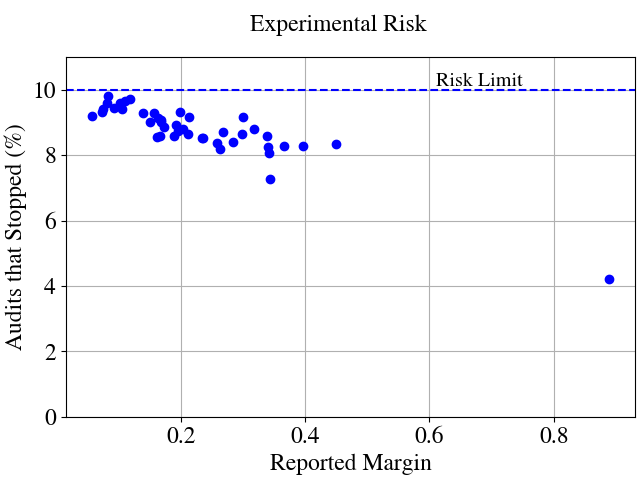
\includegraphics[width=.5\textwidth]{prov_risk.png}
\caption{The proportion of simulated audits with an underlying tie that stopped in one of the five simulated rounds.}
\label{fig:prov-risk}
\end{figure}

\begin{figure}
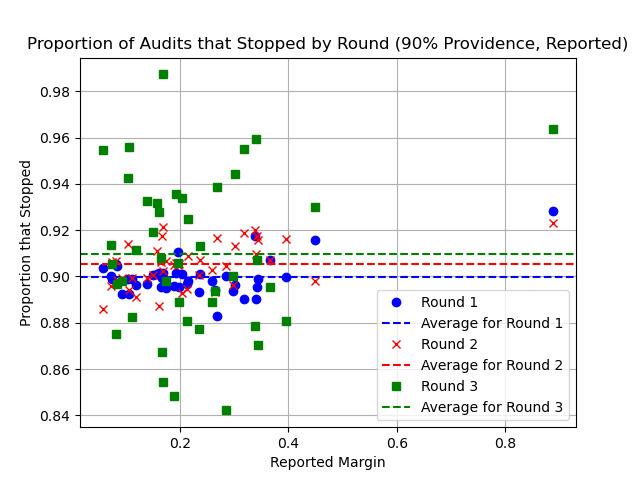
\includegraphics[width=.5\textwidth]{prov_sprob.png}
\caption{The proportion of simulated audits with an margin as announced that stopped in one of the five simulated rounds.}
\label{fig:prov-sprob}
\end{figure}

\begin{figure}
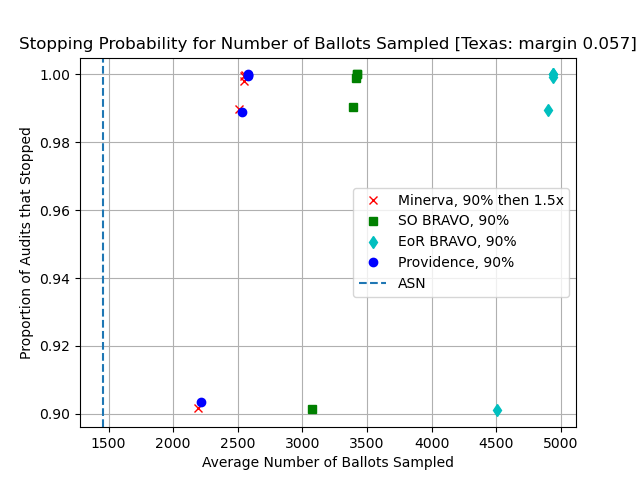
\includegraphics[width=.5\textwidth]{prov_asn.png}
\caption{For all five rounds, the estimated stopping probability for average number of ballots drawn for \Providence, \Minerva, EoR \BRAVO, and SO \BRAVO.}
\label{fig:prov-asn}
\end{figure}








